\newpage
\subsection{Card::invert() - The visual syntax}
\visHeader
\hypertarget{invertCard vis}{}

\begin{itemize}

% Make sure you explain how/why the green box. Hasn't been convered yet
\item[$\blacktriangleright$] The next SDM \emph{inverts} a card by swapping its back and face values. This therefore ``turns the card around'' in the learning box, which makes sense when
learning, for example, a new language. You're no longer an SDM beginner, so model the SDM depicted in Fig.~\ref{fig:sdm_invert}.

\begin{figure}[htbp]
\begin{center}
  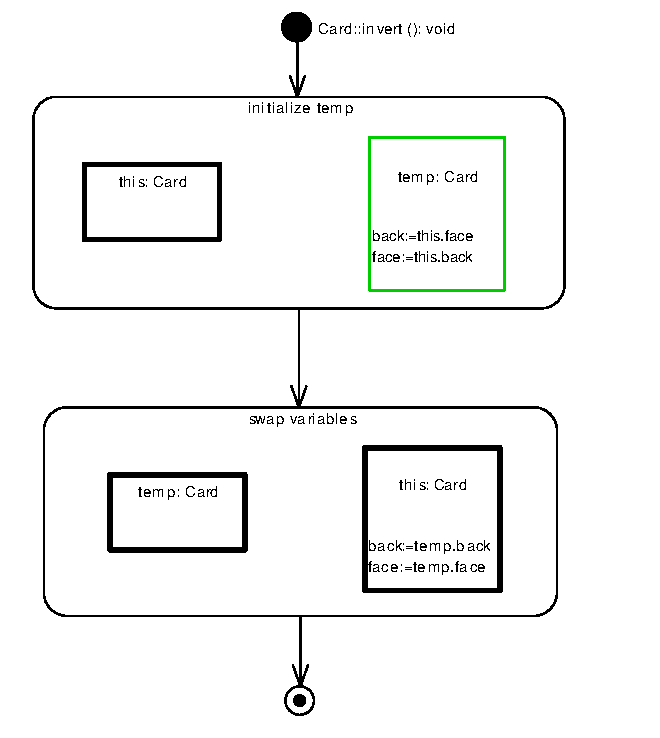
\includegraphics[width=0.6\textwidth]{ea_swappingCard.pdf}
  \caption{Swap back and face of the card.}  
  \label{fig:sdm_invert}
\end{center}
\end{figure}

\end{itemize}
